\documentclass[lettersize,journal]{IEEEtran}
\usepackage{amsmath,amsfonts}
\usepackage{algorithmic}
\usepackage{array}
\usepackage[caption=false,font=normalsize,labelfont=sf,textfont=sf]{subfig}
\usepackage{textcomp}
\usepackage{stfloats}
\usepackage{url}
\usepackage{verbatim}
\usepackage{graphicx}
\usepackage{gensymb}
\hyphenation{op-tical net-works semi-conduc-tor IEEE-Xplore}
\def\BibTeX{{\rm B\kern-.05em{\sc i\kern-.025em b}\kern-.08em
    T\kern-.1667em\lower.7ex\hbox{E}\kern-.125emX}}
\usepackage{balance}
\begin{document}
\title{Webasto ThermoTop C Controller Replacement -- Hardware}
\author{Gavin Hurlbut
\thanks{Manuscript created February, 2023; This work is based on a template that was developed in October, 2020 by the IEEE Publication Technology Department.  This work is distributed under the \LaTeX \ Project Public License (LPPL) ( http://www.latex-project.org/ ) version 1.3. A copy of the LPPL, version 1.3, is included in the base \LaTeX \ documentation of all distributions of \LaTeX \ released 2003/12/01 or later. The opinions expressed here are entirely that of the author. No warranty is expressed or implied. User assumes all risk.}}

\markboth{Journal of Beirdo's Designs, Vol. 1, No. 1, February 2023}%
{Webasto ThermoTop C Controller Replacement -- Hardware}

\maketitle

\begin{abstract}
Insert abstract here once I'm done
\end{abstract}

\begin{IEEEkeywords}
Webasto, ThermoTop C, mainboard, hardware.
\end{IEEEkeywords}


\section{Introduction}
\IEEEPARstart{T}{his} introduction will need filling in once I have sufficient text spew to do so.

This design is composed of several boards, and each will be documented here in its own section, along with the core heater that this is intended to work with.

\section{Webasto ThermoTop C}

\noindent The Webasto ThermoTop C is a coolant heater that is either fueled with gasoline or diesel fuel.  As all of my vehicles are diesel-powered, I am only really interested in the diesel models, but other than changing of some control firmware (and the corresponding fuel nozzles, etc) the same design covers both fuel types.  See figure \ref{webasto-stock} for an image of the heater.  Its purpose is two-fold: as a "parking heater", and as an "auxiliary heater".  

As a "parking heater", its job is to heat and circulate the coolant in a parked vehicle, to provide interior heat, and also to pre-warm the engine to help with starting on cold days.  Heating the engine block via cycling warmed coolant is gentler on the engine block than a plugin electric block heater, and additionally doesn't require a 120VAC circuit.

As an "auxiliary heater", the purpose is to heat the coolant immediately after the engine has been started.  This allows the engine to get to temperature faster, reducing the wear and tear, and also allowing for cabin heat earlier.  A diesel engine can often take up to tens of minutes to warm up to the point of providing ample cabin heat, so the auxiliary heater helps fill the gaps.

\begin{figure}[!t]
\centering
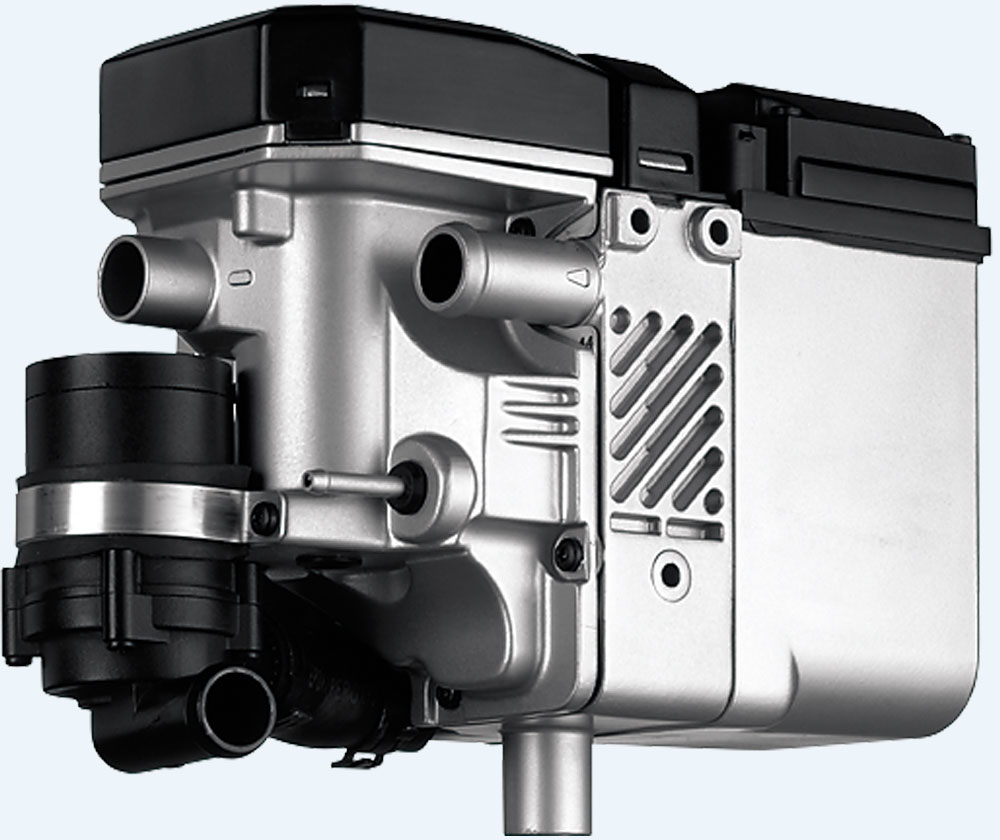
\includegraphics[width=2.5in,keepaspectratio]{Thermo-Top-C-E.png}
\caption{Webasto ThermoTop C/E}
\label{webasto-stock}
\end{figure}


\section{Webasto Replacement Controller}

\noindent Since I want slightly different behavior when using my heater, I will need to reprogram the controller that is in the heater, or replace it.  As it is highly unlikely I will be able to get the design files (hardware or firmware) of the original board (see figure \ref{controller-orig} for a view of one), I have designed my own replacement.  That is what is being documented here.

\begin{figure}[!t]
\centering
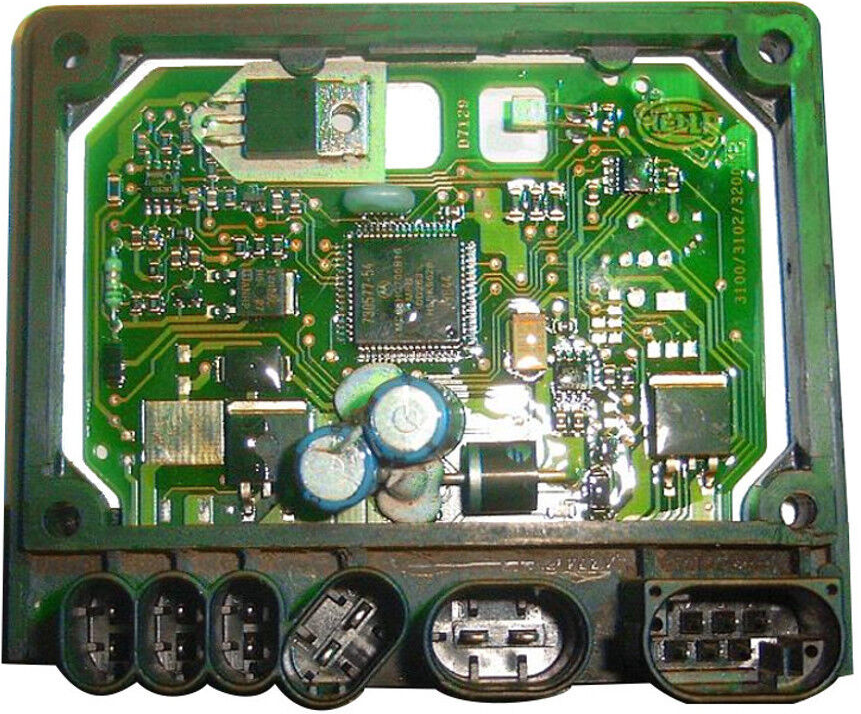
\includegraphics[width=2.5in,keepaspectratio]{mainboard-orig.png}
\caption{Webasto ThermoTop C/E OEM Controller}
\label{controller-orig}
\end{figure}

To be able to fit into the OEM frame, and use the OEM connector, great care was taken to get the shape to match the original, and to keep the connectors (at the bottom of figure \ref{controller-orig}) in the correct places and orientations.  All of the connectors other than the 6-pin X1 are used for the precisely same purpose as stock, and the majority of X1 was left in place as well.  The pinouts of these connectors are as shown in tables \ref{pinout-x1}, \ref{pinout-x2}, \ref{pinout-x3}, \ref{pinout-x4}, and \ref{pinout-x5}.

\begin{table}
\begin{center}
\caption{Pinout of Connector X1}
\label{pinout-x1}
\begin{tabular}{| c | c | c |}
\hline
Pin Number & OEM Signal & My Signal \\
\hline
1 & START & START \\
& (> 5V = ON, < 5V = OFF)  & \\
\hline
2 & K-Line/WBUS & K-Line/WBUS \\
&  Diagnostics/Control &  Diagnostics/Control \\
\hline
3 & External Thermostat & I2C SDA \\
\hline
4 & Vehicle Fan Relay + & Vehicle Fan Relay + \\
\hline
5 & Summer/Winter Switch & I2C SCL \\
\hline
6 & Fuel Dosing Pump + & Fuel Dosing Pump + \\
\hline
\end{tabular}
\end{center}
\end{table}

\begin{table}
\begin{center}
\caption{Pinout of Connector X2}
\label{pinout-x2}
\begin{tabular}{| c | c |}
\hline
Pin Number & OEM Signal \\
\hline
1 & Battery Voltage \\
& (through 15A Fuse) \\
\hline
2 & Chassis/Signal Ground \\
\hline
\end{tabular}
\end{center}
\end{table}

\begin{table}
\begin{center}
\caption{Pinout of Connector X3}
\label{pinout-x3}
\begin{tabular}{| c | c |}
\hline
Pin Number & OEM Signal \\
\hline
1 & Glow Plug + \\
\hline
2 & Glow Plug - \\
\hline
\end{tabular}
\end{center}
\end{table}

\begin{table}
\begin{center}
\caption{Pinout of Connector X4}
\label{pinout-x4}
\begin{tabular}{| c | c |}
\hline
Pin Number & OEM Signal \\
\hline
1 & Combustion Air Fan + \\
\hline
2 & Combustion Air Fan - \\
\hline
\end{tabular}
\end{center}
\end{table}

\begin{table}
\begin{center}
\caption{Pinout of Connector X5}
\label{pinout-x5}
\begin{tabular}{| c | c |}
\hline
Pin Number & OEM Signal \\
\hline
1 & Circulation Pump + \\
\hline
2 & Circulation Pump - \\
\hline
\end{tabular}
\end{center}
\end{table}

The mainboard design leverages the use of a Raspberry Pi Pico module.  This module has the RP2040 processor on it, which has two ARM Cortex-M0+ cores running at 133MHz.  At a very low price point (around \$5USD each at the time of writing), it seemed beneficial to use this as the center of it all.

To be able to have stable control loops, there are a slew of other sensors and signals that are required.  Some of these inputs were implemented on the OEM controller, but some were not.  To extend the functionality without having to further modify the enclosure, I replaced two signals on the X1 connector with I2C signals (SDA and SCL), and the sensors are on other boards, connected to the wiring harness by these two signals (plus battery voltage and ground for power).  These boards will be described further on in the document.

\subsection{Sensors}
\subsubsection{Outdoor Temperature}
Outdoor temperature is measured using a DS18B20 temperature sensor that will be remotely mounted under the vehicle, but out of the way of water splashing.  This device can measure from $-55 \degree C$ to $+125 \degree C$ (accuracy of $\mp 0.5 \degree C$ from $-10 \degree C$ to $+85 \degree C$), and is prewired and waterproofed in an assembly made by Adafruit (product 381).  This interfaces to the core CPU via 1-wire using a 1-wire to I2C bridge that is mounted on the Sensor Board.

\subsubsection{Internal CPU Core Temperature}
The RP2040 has a temperature sensor attached to ADC input 4, and it is readily accessible from Arduino using readAnalogTemperature().

\subsubsection{Battery Voltage}
Although the battery voltage is available on the mainboard, there is limited space available on it.  The battery voltage is being measured by a 12-bit ADC on the sensor board (via I2C), after being divided by about 6, giving a maximum readable voltage around 20V, which is overkill for a 12V lead acid battery, even under charge conditions.  If the battery voltage goes significantly out of spec (i.e $< 9V$ or $> 16V$), the heater will be shut down.

\subsubsection{Coolant Temperature}
The coolant temperature is measured using standard automotive coolant temperature sensors.  These are, in fact, NTC (negative temperature coefficient) thermistors which we then put into a voltage divider with a known resistance, and measure the voltage across it.  This allows us to calculate first its resistance, and from that the temperature, either by doing piecewise linear regression from a lookup table, or by doing the logarithmic math to best fit to a curve.  As the two results were very close in practise, we will use the lookup table, which is approximately 100 times faster than doing the floating point math.  These sensors give readings between $-50 \degree C$ and $+100 \degree C$.

Additionally, the coolant (and cooling water) temperatures are measured on the valve controller boards that are connected to a LINBus to I2C bridge, and thus to our I2C bus.  This allows us to sense the temperature in each of the flow loops as needed.

\subsubsection{Exhaust Temperature}
Exhaust temperature is well out of the range of the NTC Thermistor, and it appears that all of the "normal" available EGT sensors on the market are K-Type thermocouples.  We will be using a K-Type Thermocouple that connects to a special thermocouple amplifier with integrated 12-bit ADC that is on the sensor board, connected via I2C.

This sensor has a range of $-200 \degree C$ to $+1260 \degree C$.

\subsubsection{Ignition Sense}
The ignition sense is done by connecting the ignition/accessory line (usually red) to a GPIO expander after level shifting from 12V to 3.3V.  The level shifting is done using a diode which will be reverse biased when the wire is at 12V, and forward biased when the wire is grounded.  With a pull-up in place on the 3.3V side of the diode, when the wire coming from the vehicle is at 12V, the GPIO input is at 3.3V, and when it's grounded high-side, it is around 0.7V or so at the GPIO.

The ignition sense is used to know when to switch from parking heater to auxiliary heater.   When the vehicle is on, the heater will run in auxiliary mode, and when it is off, the heater will run in parking mode.

\subsubsection{Flame Detector}
The flame detector is an integral part of Webasto's original design.  To sense the heat of the flame, they use the glow plug's characteristic as a PTC (positive temperature coefficient) thermistor while it is not actively in use.  They have an expired German patent on this methodology.  Basically, the hotter the glow plug is (whether because it is activated and self-heating, or if it's being heated by a flame), the higher the resistance is.

To measure this resistance, and thus get an idea when it has cooled to far for an active flame to exist in the burn chamber, we energize the glow plug with a lower voltage and measure its voltage drop in the circuit.  To drastically simplify calculations, we will be energizing it with the help of an LM7805 linear regulator acting as a constant current source, delivering 100mA.  The voltage drop across the "detector" is measured with it taking the place of a shunt resistor, with a precision current/voltage sensor (TI's INA219) that's on the I2C bus, and located on the mainboard.

The resistance of a glow plug should normally be somewhere in the range of $100 m \Omega$ to $6 \Omega$.  If it measures less than about $2 \Omega$, we assume the flame is off.  This is done in conjunction with checking exhaust temperature, and we may end up removing the flame detector functionality at some point and rely on only the exhaust temperature to detect flameout.

\subsubsection{Start/Run Sense}
The Start/Run line is another digital signal, and is already coming in on the X1 connector.  We simply put it through level translation, and then connect it to a GPIO on the Pico module.  This signal is used to order the heater to run, and when it goes low again, the heater will be shutdown in an orderly fashion unless it has been told to start via the K-Line/WBUS interface as well.

\subsubsection{Emergency Stop Sense}
The Emergency Stop line is currently coming in on a separate onboard connector, although it might make more sense to move it to a sensor board so no modifications are needed to the housing.  Either way, it requires level translation.

When the emergency stop has been asserted (active low), the heater will be shutdown immediately, with no cooldown.  This will put the heater into a lockdown situation, but may be necessary in the case of dangerously flammable situations.

The emergency stop is also used to clear out a lockdown state by toggling it while the heater is locked down.

\subsubsection{System Voltage}
The Pico module has the VSYS (nominally +5V) rail attached to the RP2040's internal ADC on channel 3.  This is readily available in arduino using analogRead().

\subsubsection{Coolant Flow Rate}
As the desired configuration includes several bypass loops (and a cooling loop), I felt it would be useful to track how well coolant is flowing.  Each valve controller board has an attached flow meter that uses a spinning impeller with an attached hall effect sensor to send a pulse for every rotation.  Given that each rotation calculates out to a fixed volume of coolant, this allows us to measure the coolant flow.

These sensor readings are accessible via LINBus by way of the LINBus to I2C bridge and the I2C bus in general.

\subsubsection{Coolant Valve Position}
Each of the valve controller LINBus boards has two motor-driven ball valves connected to them.  These valves report when they are fully open or fully closed, and we pull this status to know when we can stop ordering the actuators to open or close. 

These sensors are accessible via LINBus by way of the LINBus to I2C bridge, and thus the I2C bus.


\subsection{Actuators}
\subsubsection{Glow Plug}
The primary purpose for the glow plug is to perform the initial ignition of the fuel which will be sprayed into the combustion chamber.  The glow plug used is apparently a "normal" ceramic glow plug.  To deliver enough current to get the plug to heat up as desired in the amount of time desired, the mainboard is feeding it from the battery by switching on a power FET (n-channel MOSFET).  This MOSFET is in turn switched on using a logic-level gate n-channel MOSFET connected to the output pin.

The output pin is actually driven by a PWM generator in the RP2040, with a duty cycle of 1-100\% (0\% is off), and the signal is further gated by an enable signal as the glow plug is also used as the flame sensor when not preheating the chamber.

\subsubsection{Fuel Dosing Pump}
The fuel dosing pump is driven by a series of narrow pulses.  Each pulse delivers a fixed amount of fuel (depending on the model of pump).  With the use of a control loop in the firmware, we drive this by bit-banging out the required waveform, with the frequency of the pulses being directly related to the amount of fuel being requested.  Other than while priming the chamber with fuel at startup time, the maximum fuel delivered is calculated to generate heat at the rated heat output of the OEM heater, and with a minimum set to just where the flame will almost go out.

Rather than the on 100\% or off 100\% type of calculations the OEM firmware appears to be using, we are attempting to modulate the fuel delivery to keep the coolant in a given range.  The requested power level is calculated out to watts and is shown on the debug screen. 

\subsubsection{Coolant Circulation Pump}
The onboard coolant circlation pump is attached to the mainboard using the X5 connector.  Since this directly drives a motor, we are using a MOSFET to deliver the required power rather than foolishly attempting to drive from a logic level gate MOSFET, or a direct GPIO on the CPU.

The circulation pump is either completely on, or completely off.  We do not attempt to modulate the pump.

\subsubsection{Cool Water Circulation Pump}
The coolant loop that is used to provide cooling on hot days also will require a pump.  This is expected to be a bilge pump or something similar.  This pump will be either completely on or completely off and we will not be attempting to modulate it.

The cool water pump is controllable over LINBus via the LINBus / I2C Bridge which resides on our I2C bus.

\subsubsection{Combustion Air Fan}
The combustion air fan is connected to the mainboard via the X4 connector.  We modulate the controlling output using a PWM Controller in the RP2040.  The control loop that controls the fuel also controls the duty cycle of the combustion air fan to add or remove air from the air/fuel mixure.  As it is a motor (again), we drive the load with a MOSFET.

\subsubsection{Vehicle Fan}
The vehicle fan output is designed to energize and deenergize a relay to turn on/off the vehicle's heat fans.  This normally would be the fans for defrosting the windshield and providing cabin heat, but in my use case, I prefer to concentrate on cabin heat only, the fan being controlled is in the rear block heater in my bus.

\subsubsection{Cooling Loop Fan}
When the cooling loop is in play and is connected to the coolant loop (via a heat exchanger), the cooling loop requires a fan on a radiator to dissipate the cabin heat to act "air-conditioning-like".  This will likely be a radiator fan that fits the chosen radiator, and will be controlled by a PWM output from the valve controller card.  Its control will be over LINBus connected via the LINBus to I2C bridge.

\subsection{I2C Bus}

As stated earlier, much of the functionality (sensors and actuators alike) are attached via the I2C bus.  This was chosen as it can connect a large number of devices to the CPU using only two IO pins.  The slight downside is that I2C relies on a fairly slow clock speed, as the standard is 100kHz or 400kHz.  Even when using the higher speed 1MHz speed, each transaction is started at 400kHz then switched over.  Only some devices are capable of doing the 1MHz speed anyways, so you can only really count on having a link that is capable of about 50kByte/s in transfer across all its nodes.

The Addresses in use in this design can be seen in table \ref{i2c-addresses}.

Address selection for each populated device on the sensor boards are programmed into the EEPROM on the board, which has an address that is indexed based on the 3 LSB of the address which are selectable per board.  This allows for a total of 8 sensor boards (including the LINBus Master board which also responds as an EEPROM).  The same A2-A0 also determine the address of the PCA9501 half used as a GPIO extender on the sensors board, and the LINBus/I2C bridge address on the LINBus Master board.  The full expected address map including the sensor boards is in table \ref{i2c-full}.

After the I2C Bus exits the mainboard on X1, a custom rewiring of the wiring harness will be needed to connect to the rest of the boards.  To simplify design, I have standardized on using the QWIIC interface standard as designed by SparkFun Electronics.  This puts +3.3V, ground, SCL and SDA onto a 1mm JST SH connector, which is very convenient for daisy-chaining signals between boards.  Thus we have the QWIIC Interface board, which connects a MOLEX 4-pin connector (VBAT, GND, SCL, SDA) to a QWIIC port, complete with its own +3.3V regulated supply.  Pullups on the SCL and SDA lines are placed on every board (mainboard, QWIIC Interface, Sensor Board, LINBus Master) to ensure good signal integrity.

Due to the Arduino Nano used on the LINBus Master being a 5V device, the SDA and SCL lines need level translation.  This is done using an N-Channel MOSFET with the gate connected to the +3.3V signal and with both the source and the drain pulled up to their respective voltage levels.  This bidirectional level translation is quick and simple and uses virtually no space.

\begin{table}
\begin{center}
\caption{I2C Device Address Map}
\label{i2c-addresses}
\begin{tabular}{| c | c | c |}
\hline
Address Range & Description & Location \\
\hline
0x18-1B & DS2482S-100+ & sensor board \\
& 1-wire to I2C Bridge & \\
\hline
0x30-37 & PCA9501 & sensor board \\
& GPIO Extender & \\
\hline
0x3C or 0x3D & 0.96" 128x64 OLED Display & external \\
& & (optional) \\
\hline
0x40-4F & INA219 & mainboard \\
& Current / Power meter & \\
\hline
0x48-4B & ADS7823 & sensor board \\
& 12-bit ADC & \\
\hline
0x50-51 & CY15E004J & mainboard \\
& 4kbit EEPROM & \\
\hline
0x60-67 & MCP96L01 & sensor board \\
& Thermocouple Interface & \\
\hline
0x70-77 & PCA9501 & sensor board \\
& 2kbit EEPROM & \\
\hline
0x70-77 & Arduino Nano & LINBus Master \\
& internal 8kbit EEPROM & \\
\hline
0x78-7F & Arduino Nano & LINBus Master \\
& LINBus/I2C bridge & \\
\hline
\end{tabular}
\end{center}
\end{table}


\begin{table}
\begin{center}
\caption{I2C Full Address Map}
\label{i2c-full}
\begin{tabular}{| c | c | c |}
\hline
Address Range & Description & Location \\
\hline
0x18 & DS2482S-100+ & sensor board 0 \\
& external temperature & \\
\hline
0x30 & PCA9501 GPIO Extender & sensor board 0 \\
& ignition sense & \\
\hline
0x31 & PCA9501 GPIO Extender & sensor board 1 \\
& unused & \\
\hline
0x32 & PCA9501 GPIO Extender & sensor board 2 \\
& unused & \\
\hline
0x3C & 0.96" 128x64 OLED Display & external \\
& (optional) & \\
\hline
0x4F & INA219 & mainboard \\
& flame detector & \\
\hline
0x48 & ADS7823 & sensor board 0 \\
& battery voltage & \\
\hline
0x49 & ADS7823 & sensor board 1 \\
& coolant temperature & \\
\hline
0x50-51 & CY15E004J & mainboard \\
& 4kbit EEPROM & \\
\hline
0x60 & MCP96L01 & sensor board 2 \\
&  exhaust temperature & \\
\hline
0x70 & PCA9501 & sensor board 0 \\
& 2kbit EEPROM & \\
\hline
0x71 & PCA9501 & sensor board 1 \\
& 2kbit EEPROM & \\
\hline
0x72 & PCA9501 & sensor board 2 \\
& 2kbit EEPROM & \\
\hline
0x73 & Arduino Nano & sensor board 3 \\
& internal 8kbit EEPROM & LINBus Master \\
\hline
0x7B & Arduino Nano & sensor board 3 \\
& LINBus/I2C bridge & LINBus Master \\
\hline
\end{tabular}
\end{center}
\end{table}



\begin{IEEEbiographynophoto}{Gavin Hurlbut}
Biography text here without a photo.
\end{IEEEbiographynophoto}


\end{document}


